% Basic stuff
\documentclass[a4paper,10pt]{article}
\usepackage[nswissgerman]{babel}
%4 stackanchor  
\usepackage{stackengine}


% 3 column landscape layout with fewer margins
\usepackage[landscape, left=0.75cm, top=1cm, right=0.75cm, bottom=1.5cm, footskip=15pt]{geometry}
\usepackage{flowfram}
\ffvadjustfalse
\setlength{\columnsep}{1cm}
\Ncolumn{3}

% define nice looking boxes
\usepackage[many]{tcolorbox}

% a base set, that is then customised
\tcbset {
  base/.style={
    boxrule=0mm,
    leftrule=1mm,
    left=1.75mm,
    arc=0mm, 
    fonttitle=\bfseries, 
    colbacktitle=black!10!white, 
    coltitle=black, 
    toptitle=0.75mm, 
    bottomtitle=0.25mm,
    title={#1}
  }
}

\definecolor{brandblue}{rgb}{0.34, 0.7, 1}
\newtcolorbox{mainbox}[1]{
  colframe=brandblue, 
  base={#1}
}

\definecolor{orange}{rgb}{1, 0.55, 0.3}
\newtcolorbox{tbox}[1]{
  colframe=orange, 
  base={#1}
}

\definecolor{green}{rgb}{0.294, 0.729, 0.254}
\newtcolorbox{bembox}[1]{
  colframe=green, 
  base={#1}
}

\definecolor{red}{rgb}{0.99, 0.04, 0.99}
\newtcolorbox{tipbox}[1]{
  colframe=red, 
  base={#1}
}

\newtcolorbox{defbox}[1]{
  colframe=black!20!white,
  base={#1}
}



% Mathematical typesetting & symbols
\usepackage{amsthm, mathtools, amssymb} 
\usepackage{marvosym, wasysym}


\allowdisplaybreaks

% Tables
\usepackage{tabularx, multirow}
\usepackage{booktabs}
\renewcommand*{\arraystretch}{2}

% Make enumerations more compact
\usepackage{enumitem}
\setitemize{itemsep=0.5pt}
\setenumerate{itemsep=0.75pt}

% To include sketches & PDFs
\usepackage{graphicx}

% For hyperlinks
\usepackage{hyperref}
\hypersetup{
  colorlinks=true
}
% Math helper stuff
\def\limn{\lim_{n\to \infty}}
\def\limxo{\lim_{x\to 0}}
\def\limxi{\lim_{x\to\infty}}
\def\limxn{\lim_{x\to-\infty}}
\def\sumk{\sum_{k=1}^\infty}
\def\sumn{\sum_{n=0}^\infty}
\def\R{\mathbb{R}}
\def\dx{\text{ d}x}

\title{Analysis Cheatsheet}
\author{Konstantin Lucny}
\date{June 2023}

\begin{document}
%\maketitle



\section{Reelle \& komplexe Zahlen}
\subsection{Reelle Zahlen}

\subsection{Komplexe Zahlen}
\subsubsection{Polarform}
$ x = r\cos {\varphi};\ y=r\sin{\varphi};\  $ $r=|z|=\sqrt{x^2+y^2}$\\
$z=x+iy=r(cos(\varphi)+sin(\varphi))=re^{i\varphi} $\\
$\varphi=\arccos{\bigg(\dfrac{x}{r}\bigg)} \leftarrow$  nicht immer definiert,\\
da es auf den Quadranten drauf ankommt
\subsection{Konjugation}
$\overline{e^z}=e^{\overline{z}}$ (z.B. $\overline{e^{ix}}=e^{-ix}$)
\begin{tbox}
    {Satz 1.3.4: Fundamentalsatz der Algebra}
    Sei $n\ge 1, n\in \mathbb N$ und $P(z)=z^n+a_{n-1}z^{n-1}+...+a_0, a_j\in \mathbb C$; Dann gibt es $z_1,...,z_n \in \mathbb C$, s.d. $P(z)=(z-z_1)(z-z_2)...(z-z_n)$. Die Menge $\{z_1,...,z_n\}$ und die Vielfachheit der Nullstellen $z_j$, d.h., die Anzahl der Zahlen $k$ sodass $z_k=z_j$, sind eindeutig bestimmt.
\end{tbox}

%  Kapitel 2
\section{Folgen \& Reihen}
\subsection{Grenzwert}
\begin {defbox}{Definition Grenzwert: } $a \in \R $ ein Grenzwert von $(a_n)_{n\in \mathbb{N}};\\ \forall \epsilon > 0, \exists \text{N} \in \mathbb{N}, \text{ sodass } |a_n-a|<\epsilon, \forall n \in N $ 
\end {defbox}
\begin{defbox}{Definition: Folge} Eine Folge reeller Zahlen (bzw. komplexer Zahlen) ist eine Abbildung $\mathbb{N} \longrightarrow \mathbb{R} $ (bzw. $\mathbb{N}\longrightarrow\mathbb{C}$)
$(a_n)_{n\in \mathbb{N}}=(a_1,a_2,a_3,...,a_n)=$n-tes Folgeglied
\end{defbox}
\begin{tbox}{Hilfsatz 2.1.3}
Sei $(a_n)_{n\in\mathbb{N}}$ eine Folge \underline{reeller} Zahlen. Es gibt höchstens eine reelle Zahl $l$, sodass: $\forall y>0$, gibt es nur endlich viele $n\in \mathbb{N}$ mit $|a_n-l|\ge y$
\end{tbox}

\begin{defbox}{Definition 2.1.4: Konvergenz einer Folge}
Die Folge $(a_n)$ konvergiert falls eine Zahl $l$ existiert mit der Eigenschaft oben, $l$ ist dann eindeutig, und ist der \underline{Grenzwert} der Folge, bezeichnet 
$l=\lim_{n\to +\infty}(a_n)$ oder $a_n\longrightarrow_{n\to +\infty} l$\\
Falls $(a_n)$ nicht konvergent ist, ist sie \textbf{divergent}.
\end{defbox}

\begin{bembox}{Bemerkung}
\begin{enumerate}
    \item Die Existenz des Grenzwerts gilt nicht für alle Folgen! die Notation "$\lim(a_n)$" kann \underline{nur} benutzt werden, wenn man überprüft hat dass der \textbf{Grenzwert existiert}!
    \item Eine Menge $ A  \subset \mathbb{N}$ ist endlich $\iff$ es gibt $N\in \mathbb{N}$ sodass $ (n\ge N \implies n\notin A) $\\
    \textbf{D.h.} $\lim_{n\to\infty}(a_n)\iff\forall y >0, \exists N \in \mathbb{N}, \forall n \ge N, |A_n-l|< y$ 
    \item "$\forall y > 0 $" nur für "kleine$"$ $y$ wichtig
    \item Existenz von $\lim(a_n)$ hängt von $a_n$ für n gross genug ab.
\end{enumerate}
\end{bembox}

\begin{tbox} {Hilfssatz}
Jede konvergente Folge ist beschränkt. D.h. $\exists C \ge 0, \forall n \in \mathbb{N}, |a_n|\le C\iff \exists C \ge 0, \forall n \in \mathbb{N}, |a_n|\in [-C,C]$
\end{tbox}
\begin{bembox}{Bemerkung}
    \begin{enumerate}
        \item $\big((a_n\longrightarrow_{n\to\infty} l) \iff (|a_n-l|\longrightarrow_{n\to\infty} 0)$ und $(b_n)$ konvergiert gegen $0\big)\iff (\forall y > 0, \exists N \in \mathbb{N}, \forall n\ge N, |b_n|<y)$
        \item "\underline{Vergleichsprinzip}": falls $(c_n)$ konvergiert gegen $0$ und $0\le |a_n| \le c_n$, dann folgt $a_n\longrightarrow 0$
    \end{enumerate}
\end{bembox}
\begin{tbox}{Satz 2.1.8}
    Seien $(a_n), \ (b_n) $ konvergente Folgen mit \\$a=\lim a_n, \ b= \lim b_n$
     \begin{enumerate}
         \item $(a_n+b_n)_{n\in\mathbb{N}} \longrightarrow a+b$ 
         \item $(a_n\cdot b_n)_{n\in \mathbb N} \longrightarrow a\cdot b$ 
         \item Falls $b\neq 0$, ist $b\neq 0$ für $n$ gross genug (z.B. $n\ge N$) und $\bigg(\dfrac {a_n} {b_n}\bigg)_{n\ge N}\longrightarrow \dfrac a b $
         \item Falls $a_n\le b_n$ für alle $n$, ist $a\le b$
     \end{enumerate}
\end{tbox}
\begin{flushleft}
\textbf{Vorsicht: } $a_n<b_n$ für $n\in \mathbb N$ impliziert nicht dass $a<b$!
\end{flushleft}

\begin{tbox}{Sandwichsatz}
$(a_n)_{n\in\mathbb N}, (b_n)_{n\in\mathbb N}$ konvergent, $\forall n; a_n\le b_n \implies \lim_{n\to\infty} (a_n)\le \lim_{n\to\infty}(b_n)$. \\Es folgt direkt $(a_n)_{n\in\mathbb{N}},(b_n)_{n\in\mathbb{N}}, (c_n)_{n\in\mathbb{N}}$ konvergent und $a_n\le b_n \le c_n, \forall n \ge N$ und $\lim_{n\to\infty}(a_n)=\lim_{n\to\infty}(c_n)=l\implies \lim_{n\to\infty}(b_n)=l$
    
\end{tbox}

\subsection{Monotone Folgen}
\begin{tbox}{Satz 2.2.2: Monotonie einer Folge}
    Sei $(a_n)$ eine Folge reeller Zahlen:
    \begin{enumerate}
        \item Falls $(a_n)$ \underline{wachsend} ist (d.h. $\forall n\in \mathbb N, a_{n+1}\ge a_n$ ist sie \underline{konvergent}$\iff C\ge 0 $, sodass $\forall n \in \mathbb N, a_n \le C$.
        Der Grenzwert ist $\lim(a_n) = \sup\{a_n|n\in\mathbb N \} (\le C)$
        \item Falls $(a_n)$ \underline{fallend} ist $(a_{n+1}\le a_n $ für $n\in \mathbb N $, ist $(a_n)$ konvergent $\iff$ es gibt $C\in \mathbb R$ sodass $\forall n \in \mathbb N,\ a_n\ge C$, und dann $ \lim(a_n)=\inf\{a_n|n\in \mathbb N\}$
    \end{enumerate}
\end{tbox}

\begin{defbox} {Definition Konvergent}
Sei $(a_n)$ eine Folge reeller Zahlen $a_n\longrightarrow l  \in \mathbb R \iff \forall y > 0, \exists N \in \mathbb N, \forall n \ge N, |a_n-l|<y$
\end{defbox}
\begin{tipbox}{Trick}
    Warum ist $l=\lim(a_n)=\lim_{n\to\infty}(n^a q^n)=0$?\\
    $\frac{a_{n+1}}{a_n}=\underbrace{(1+\frac{1}{n})^a}_{\to 1} \underbrace{q}_{\to q}$
    \\ $\lim(a_{n+1})=\lim(a_n)=l \implies ($wenn $ l\neq 0 \implies \frac{a_{n+1}}{a_n}=1) $
    \\ Da $1=q $ unmöglich, folgt $l=0$
\end{tipbox}
\begin{bembox}{Schnelle Konvergenz}
    Die Konvergenz ist $"$sehr schnell$"$ für die Folge, die gegen die Quadratwurzel von $a_1$ geht.
\end{bembox}

\subsection{Liminf \& Limsup}
\begin{defbox}{Definition: Liminf \& Limsup}
    Sei $(a_n)$ eine Folge reeller Zahlen die \underline{beschränkt} ist: $\exists M \in \mathbb R, \forall n \in \mathbb N, |a_n|\le M$
    \\ Wir definieren Folgen $(b_k)_{k\in \mathbb N}, (c_k)_{k\in \mathbb N}$ durch:
    \begin{center}
        Sei $k \in \mathbb N$:
        $X_k=\{a_n|n\ge k\}\subset \mathbb R$
        \\ $\forall k, \ X_k\subset [-M,M]$ und $X_k\neq \emptyset \ (a_k \in K_k)$ 
        \\ $\implies X_k$ hat ein Supremum $c_k$ und ein Infimum $b_k$
        \\ Das bedeutet insb.: $\forall n \ge k, b_k\le a_n \le c_k$
        \\ Sei $k\in \mathbb N:$ es gilt $X_{k+1}\subset X_k\implies
        \begin{cases}
            b_{k+1}\ge b_k (Infimum)\\
            c_{k+1}\le c_k (Supremum)
        \end{cases}
        $
        Folgend gilt: 
        \begin{itemize}
            \item $(b_k)$ ist \underline{wachsend} und $b_k\le M$ für $k\in \mathbb N (b_k=\inf(X_k)$ und $X_k\subset [-M,M])$
            \item $(c_k)$ ist \underline{fallend} und $c_k\ge -M$ für $k\in \mathbb N \ (c_k=\sup(X_k)$
        \end{itemize}
    \end{center}
\end{defbox}
\begin{flushleft}
    \textbf{Vorsicht:} $\liminf(a_n+b_n)$ oder $\limsup(a_n+b_n)$ ist \underline{nicht immer} $\liminf(a_n)+\liminf(b_n)$. Gleiches gilt bei \underline{Multiplikation}.
\end{flushleft}

\subsection{Das Cauchy Kriterium}
\begin{tipbox}{Anleitung für Cauchy Kriterium}
    \begin{enumerate}
        \item Schritt: $(a_n)$ reelle Folge konvergiert $\iff (a_n)$ beschränkt und $\liminf(a_n)=\limsup(a_n)$
        \item Schritt: 
        \begin{tbox} {Satz 2.4.2: Cauchy Kriterium}
            Eine Folge $(a_n)$ reeller Zahlen konvergiert $\iff \forall y>0, \exists N \in \mathbb N, \\ 
            \forall m\ge N, \forall n \ge N, |a_m-a_n|<y$ 
        \end{tbox}
        \begin{bembox}{Bemerkung}
            Dies ist auch eine Version der \underline{Vollständigkeit} von $\mathbb R$
        \end{bembox}
    \end{enumerate}
\end{tipbox}
% \begin{bembox}{Bemerkung}
% $a_n=1+\frac{1}{2^3}+\frac{1}{3^3}+...+\frac{1}{n^3}$ konvergiert; ob $\lim(a_n)$ etwas mit $\pi$ zu tun hat weiss man \underline{nicht}!
    
% \end{bembox}

\subsection{Satz Bolzano-Weierstrass}

\begin{tbox} {Definition Bolzano-Weierstrass (Übungsst.)}
$(a_n)_{n\in\mathbb N}$ eine Folge mit $a_{n+1}\ge a_n, \forall n$ (monoton wachsend) und die Folge ist von oben beschränkt $\implies (a_n)_{n\in\mathbb N}$ konvergiert.
\end{tbox}

\begin{tbox}{Definition Bolzano-Weierstrass}
Jede \underline{beschränkte} Folge hat mindestens eine konvergent Teilfolge (z.B. $a_n=(-1)^n 
\begin{cases}
    a_{2n} \longrightarrow 1
    \\a_{2n+1} \longrightarrow -1
\end{cases})$
\end{tbox} 
\begin{defbox} {Definition Teilfolge}
    Sei $(a_n)_{n\in\mathbb N}$ eine Folge. Eine Folge $(b_k)_{k\in\mathbb N}$ heisst \underline{Teilfolge} von $(a_n)$ wenn es gibt $t:\mathbb N \longrightarrow \mathbb N$, sodass 
    $\begin{cases}
        (1) & b_k=a_{t(k)}
        \\(2) & t(k+1)>t(k)
    \end{cases}$
\end{defbox}

\begin{defbox} {Definition Häufungspunkt}
    \begin{enumerate}
        \item Fall: $(a_n)$ Folge; $(b_k)$ konvergierte Teilfolge, $l=\lim(b_k)$ von $(a_n)$ Man sagt $l$ ist \underline{ein} \textbf{Häufungspunkt}.
        \item Fall: $(a_n)$ konvergent ist, mit $\lim_{n\to\infty}(a_n)=l$, jede Teilfolge von $(a_n)$ konvergiert mit Grenzwert $l \implies$ \underline{nur} $l$ ist ein \textbf{Häufungspunkt}
        \item Fall: Es kann sein, dass $(a_n)$ \underline{unendlich viele} \textbf{Häufungspunkte} hat (z.B. $\cos$).
    \end{enumerate}    
\end{defbox}

\subsection{Folgen in $\mathbb C$ (oder $\mathbb R^d$) und Grenzwerte $+\infty, -\infty$}
\begin{defbox}
    {Definition: Folge komplexer Zahlen}
    $(a_n)_{n\in\mathbb N}$ Folge von komplexer Zahlen: $a_n = b_n + ic_n$
    $a_n$ ist durch zwei Folgen reeller Zahlen bestimmt.
\end{defbox}
\begin{tbox}
    {Satz: komplexe Folgen}
    Sei $a_n=b_nic_n\in\mathbb C$ und $l=u+iv\in\mathbb C$
    Folgende Eigenschaften sind äquivalent:
    \begin{enumerate}
        \item $\forall \epsilon>0, \exists N\in\mathbb N, \forall n \ge N, |a_n-l|<\epsilon$
        \item $(|a_n-l|)_{n\in\mathbb N}$ konvergiert gegen $0$
        \item $b_n\longrightarrow u \ \big(=\Re(a_n)\longrightarrow\Re(l)\big)$ und $c_n\longrightarrow v \ \big(=\Im(a_n)=\Im(l)\big)$
    \end{enumerate}
         Dann sagt man, dass $(a_n)\longrightarrow l, \ \lim(a_n)=l$
\end{tbox}

\begin{bembox}
    {Bemerkung}
    Fast alles was für reelle Folgen gilt, gilt auch für komplexe, mit Ausnahme \underline{kein} $\liminf$ oder $\limsup$.
\end{bembox}

\begin{tbox}
    {Satz: Kombination komplexer Limits}
    \begin{enumerate}
        \item $a_n\longrightarrow l \in \mathbb C$ und $b_n\longrightarrow l'\in \mathbb C$ $\implies$ $a_n+b_n \longrightarrow l+ l'$ und $a_n\cdot b_n \longrightarrow l \cdot l'$ sowie falls $ l'\neq 0$, $\dfrac{a_n}{b_n}\longrightarrow \dfrac{l}{l'}$ [$b_n\neq 0$ für $n$ gross genug]
        \item $a_n \longrightarrow l \iff |a_n-l|\longrightarrow 0$
        \item $(|a_n|\le b_n$ und $b_n\longrightarrow 0) \implies a_n \longrightarrow 0$
    \end{enumerate}
\end{tbox}

\begin{tbox}
    {Satz 2.6.6: Cauchy \& Bolzano-Weierstrauss}
    Sei $(a_n)$ Folge \underline{komplexer} Zahlen
    \begin{enumerate}
        \item Cauchy Kriterium: $(a_n) $ konvergiert $\iff \forall \epsilon >0, \exists N\in \mathbb N, \forall n, \forall m, (n\ge N, m\ge N \implies |a_n-a_m|<\epsilon)$
        \item Bolzano-Weierstrauss: Falls $(a_n)$  \underline{beschränkt} ist, gibt es (mindestens) eine konvergente Teilfolge.
    \end{enumerate}
\end{tbox}

\begin{defbox}
    {Definition: Konvergenz gegen $\pm\infty$}
    Sei $(a_n)$ eine Folge reeller Zahlen. Die Folge $(a_n)$ konvergiert gegen $+\infty \iff \forall A\in \mathbb R, \exists N \in \mathbb N, \forall n \ge N, a_n > A$ (bzw. $a_n<A$)
\end{defbox}
\begin{bembox}
    {Bemerkung}
    Eine unbeschränkte Folge ist \underline{nicht immer} gegen $\pm\infty$ konvergent.
\end{bembox}
\begin{tbox}
    {Satz: Beschränkung monotoner Folgen}
    Falls $(a_n)$ wachsend (bzw. fallend) ist, gilt:
    \begin{enumerate}
        \item entwerder ist $(a_n)$ \underline{beschränkt} und konvergiert
        \item oder $(a_n)$ ist \underline{unbeschränkt} und $a_n\longrightarrow+\infty$ (bzw. $a_n\longrightarrow -\infty$)
    \end{enumerate}
\end{tbox}
\begin{tbox}
    {Satz: Kombination Limits (eine Folge gegen $+\infty$)}
    $(a_n),\ (b_n) Folgen, b_n \longrightarrow+\infty:$
    \begin{enumerate}
        \item Falls $(a_n)$ beschränkt ist, gilt $a_n+ b_n \longrightarrow+\infty$
        \item Falls $a_n\longrightarrow l$, folgt $\dfrac{a_n}{b_n}\longrightarrow 0$
        \item Falls $a_n\longrightarrow 0, \ a_n >0, \ \dfrac{1}{a_n}\longrightarrow +\infty$
    \end{enumerate}
\end{tbox}
\begin{tipbox}
    {Limits Polynomdivision}
    Seien $p(x)=a_dx^d+a_{d-1}x^{d-1}+...+a_0\ (a_d\neq 0)$ und $(q(x)=b_cx^c+b_{c-1}x^{c-1}+...+b_0\ (b_c\neq 0)$ 
    \\\underline{Bem:} für $n$ gross genug ist $q(n)\neq 0$.
    \begin{enumerate}
        \item $d>c$: $\lim \dfrac{p(n)}{q(n)}=\pm \infty$ $(+\infty[$bzw.$\ -\infty] $ genau dann wenn $\dfrac{a_d}{b_c}>0[$bzw. $<0]$
        \item $d=c$: $\lim_{n\to \infty} \dfrac{p(n)}{q(n)}=\dfrac{a_d}{b_c}=\dfrac{a_d}{b_d}\ (\neq 0)$
        \item $d<c$: $\lim_{n\to \infty}\dfrac{p(n)}{q(n)}=0$
    \end{enumerate}
\end{tipbox}
\subsection{Reihen}
\begin{defbox}
    {Definition Reihen}
    Die Folge $(a_n)$, wo $a_n=x_0+...+x_n$, ist die Folge der partiellen \underline{Summen} der Reihe mit Gliedern $(x_n)_{n\ge0}$, bezeichnet $\sum_{n=0}^{+\infty}x_n$
\end{defbox}
\begin{bembox}
    {Bemerkung}
    \begin{enumerate}
        \item \textbf{\underline{Nur}} wenn die Folge $(a_n)$ konvergiert, ist der Grenzwert die Summe der Reihe: $\sum_{n=0}^{+\infty}x_n=lim_{n\to\infty}a_n$
        \item Grenzwert ist \underline{schwer} zu berechnen (auf bekannte Reihen zurückführen)
    \end{enumerate}
\end{bembox}
\begin{defbox}
    {Definition: Absolute Konvergenz}
    $\sum_{n=0}^{\infty}a_n$ konvergiert absolut falls $\sum_{n=0}^\infty|a_n|$ konvergiert.
    \begin{enumerate}
        \item absolute Konvergenz $\implies$ Konvergenz
        \item Falls $a_n\ge 0$: Konvergenz $\iff$ absolute Konvergenz
    \end{enumerate}
\end{defbox}
\begin{tbox}
    {Konvergenzkriteren (aus der Übung)}
    \begin{enumerate}
        \item \underline{Leibnitzkriterium} (bei alternierenden Folgen): Falls $(a_n)_n$ monoton fallend \& $\lim_{n\to \infty}(a_n)=0$, dann konvergiert $\sum_{n=0}^\infty(-1)^na_n$
        \item \underline{Vergleichkriterium}: 
        \begin{itemize}
            \item Falls $\sum_{n=0}^\infty|b_n|$ konvergiert und $\exists N$: $|a_n|\le|b_n|,\ \forall n\ge N$. Dann konvergiert $\sum_{n=0}^\infty|a_n|$ absolut.
            \item Falls $\sum_{n=0}^\infty|b_n|$ divergiert und $\exists N$: $|b_n|\le|a_n|\forall n \ge N$ Dann divergiert $\sum_{n=0}^\infty|a_n|$
        \end{itemize}
        \item \underline{Quotienten Kriterium} ($\limsup$ und $\liminf$ durch $\lim$ ersetzt: $\sum_{n=0}^\infty a_n$ eine Reihe. $d=\lim_{n\to\infty}\dfrac{|a_{n+1}|}{|a_n|}$ (falls es existiert)
        \begin{itemize}
            \item $d<1$: Reihe konvergiert
            \item $d>1$: Reihe divergiert
            \item $d=1$: Keine Aussage
        \end{itemize}
        \item \underline{Wurzelkriterium}: $\sum_{n=0}^\infty a_n$ eine Reihe, $d=\lim_{n\to\infty}\sqrt[n]{|a_n|}$
        \begin{itemize}
            \item $d<1$: absolut konvergent
            \item $d>1$: divergent
        \end{itemize}
    \end{enumerate}
\end{tbox}
\begin{defbox}
    {Definition: Zeta-Funktion}
    $\sum_{n=1}^\infty \dfrac{1}{n^s}$ divergiert für $s\le 1$ und konvergiert für $s>1$.
\end{defbox}
\begin{tipbox}
    {Intuition: Konvergenz von Reihen}
    $\sum_{n=0}^{+\infty}x_n$ konvergiert wenn $ (x_n)$ konvergiert $"$schnell genug$"$ gegen $0$.
\end{tipbox}
\begin{tbox}
    {Satz 2.7.4/2.7.5/2.7.6}
    Seien $(x_n)_{n\ge 0} >(y_n)_{n\ge0}$ Folgen komplexer Zahlen:
    \begin{enumerate}
        \item $\sum_{n=0}^{+\infty} (x_n+y_n)=\sum_{n=0}^{+\infty} x_n+\sum_{n=0}^{+\infty} y_n$, falls $\sum_{n=0}^{+\infty} x_n$ \& $\sum_{n=0}^{+\infty} y_n$ konvergieren.
        \item $\sum_{n=0}^{+\infty} (x\cdot x_n) = x \cdot\sum_{n=0}^{+\infty} x_n$, falls $x\in \mathbb C$ und $\sum_{n=0}^{+\infty}x_n$ konvergiert.
        \item Cauchy Kriterium: $\sum_{n=0}^{+\infty} x_n$ konvergiert $\iff \forall \epsilon >0, \exists N\ge0, \forall m\ge n\ge N, 
        \\\bigg|\sum_{k=n+1}^{m} x_k \bigg|<\epsilon$
        \item Sei $x_n\ge 0$, die Reihe $\sum_{n=0}^{+\infty}x_n$ konvergent (gegen eine Zahl) $\exists C \in \mathbb R, \ \forall n \in \mathbb N,\ 0\le x_o+...+x_n\le C$
    \end{enumerate}
\end{tbox}
\begin{defbox}
    {Definition 2.7.9: Konvergenz einer komplexer Folge}
    Sei $(x_n)$ eine komplexe Folge. Die Reihe $\sum_{n=0}^{+\infty}$ konvergiert \underline{absolut} falls $\sum_{n=0}^{+\infty}|x_n|$ konvergiert.
\end{defbox}
\begin{tbox}
    {Satz 2.7.10: Reihe Konvergenz gegen Zahl}  
    Jede Reihe $\sum_{n=0}^{+\infty}x_n$ die absolut konvergent ist, \underline{konvergiert} (gegen eine Zahl) und $\big|\sum_{n=0}^{+\infty}x_n\big|\le\sum_{n=0}^{+\infty}|x_n|$ (gehört $\mathbb R$, weil $\sum_{n=0}^{+\infty}x_n$ konvergiert absolut)
\end{tbox} 
\begin{tbox}
    {Satz 2.7.12: Reihe Konvergenz gegen Zahl}
    Sei $(a_n)_{n\ge0}$ fallend, $ a_n\ge 0, \ a_n\longrightarrow 0$ Die Reihe $\sum_{n=0}^{+\infty}(-1)^na_n$ ist dann konvergent (\underline{gegen eine Zahl})
\end{tbox}
\begin{tbox}
    {Satz 2.7.16: Umordnen einer Reihe}
    Fall $\sum x_n$ \underline{absolut} konvergent ist, kann man sie umordnen "wie man will". Summe bleibt \underline{gleich}.
\end{tbox}
\begin{flushleft}
    \textbf{Vorsicht}: eine Reihe die \underline{nicht} absolut konvergent ist (aber konvergent) kann man nicht umordnen wie man will!
\end{flushleft}
\begin{bembox}
    {Bemerkung}
    Falls $\sum x_n$ konvergiert und $x_n\in\mathbb R$, nicht absolut, ist \underline{jede} reelle Zahl die Summe einer umgeordneten Reihe.
\end{bembox}
\begin{defbox}
    {Definition: $\exp(z)$}
    Sei $z\in\mathbb C$: $e^z=\exp(z)=\sum_{n=0}^{+\infty}\dfrac{z^n}{n!}$ \\
     $e^x>= x+1$
\end{defbox}
\begin{defbox}
    {Definition: Potenzreihen}
    Wir überlegen $(x_n)_{n\in\mathbb N}$, komplexe Folge, und für jedes $z\in \mathbb C$, die Reihe $\sum_{n=0}^{+\infty}x_nz^n$.
\end{defbox}
\begin{tbox}
    {Korollar 2.7.21: Konvergenz Potenzreihe}
    Nur \underline{eine} der folgenden Möglichkeiten gilt:
    \begin{enumerate}
        \item für $z\neq 0,\ \sum x_nz^n$ divergiert. Konvergenzradius $r=0$
        \item für alle $z\in\mathbb C,\ \sum x_n,z^n$ konvergiert \underline{absolut} $\implies$ $"$ Konvergenzradius $r=+\infty"$
        \item es gibt $r\in ]0,+\infty[$, sodass
        \begin{itemize}
            \item $\sum_{n=0}^{+\infty}x_nz^n$ \underline{konvergiert absolut} für $|z|<r$
            \item $\sum_{n=0}^{+\infty}x_nz^n$ \underline{divergiert} für $|z|>r$
        \end{itemize}
    \end{enumerate}
\end{tbox}
\begin{defbox}
    {Definition 3.7.10: Konvergenzradius}
    Die Potenzreihe $\sum_{n=0}^{+\infty}c_nz^n$ hat \underline{positiven} Konvergenzradius,\\
    falls $\limsup_{n\to\infty}\sqrt[n]{|c_n|}$ exisitiert.    
    $$r=
    \begin{cases}
    
        \hfil +\infty & falls \ \limsup_{n\to\infty}\sqrt[n]{|c_n|}=0
        \\ \dfrac{1}{\limsup_{n\to\infty}\sqrt[n]{|c_n|}} & falls \ \limsup_{n\to\infty}\sqrt[n]{|c_n|}>0
    \end{cases}$$

    
\end{defbox}

\begin{tbox}
    {Korollar 2.7.29:  Vertauschung zweier Grenzwerte von $\exp{z}$}
    Sei $z\in\mathbb C$. Es gilt: $\exp{(z)}=\sum_{n=0}^{+\infty}\underbrace{\dfrac{z^n}{n!}}_{=\lim_{m\to\infty}x_{m,n}}=\lim_{n\to\infty}(1+\dfrac z m )^m$\\
    Insbesondere: $e=\exp{(1)}=\lim_{m\to\infty}(1+\frac 1 m)$ (folgt aus der erlaubten Vertauschung zweier Grenzwerte.
\end{tbox}

\begin{tbox}
    {Satz 2.7.23: Doppelreihen}
    Seien $(x_{m,n})_{m,n\in\mathbb N}$ komplexe Zahlen. Wir nehmen an: es gibt $C\ge0$, sodass für alle $M,N\in \mathbb N,\ \sum^M_{m=0}\sum_{n=0}^N|x_{m,n}|\le C, \forall m \ge 0$. Dann sind alle Zeilen/Spalten Reihen konvergent und $$\sum^{+\infty}_{m=0}\sum_{n=0}^{+\infty}|x_{m,n}|=\sum^{+\infty}_{n=0}\sum_{m=0}^{+\infty}|x_{m,n}|$$
    Beide Reihen sind absolut konvergent.
\end{tbox}
\begin{tbox}
    {Satz 2.7.26: Rechnen konvergenten Reihen}
    Falls $\sum_{m=0}^{+\infty}x_m,\ \sum_{n=0}^{+\infty}y_n$ absolut konvergente Reihen mit $x_m,\ y_n\in \mathbb C$ sind, ist $$(\displaystyle\sum_{m=0}^{+\infty}x_m)(\displaystyle\sum_{n=0}^{+\infty}y_n)= \displaystyle\sum_{n=0}^{+\infty}(\displaystyle\sum_{m=0}^{n}x_{n-m}\cdot y_m)$$
\end{tbox}
% \begin{bembox}
%     {Notation: $\exp{(z)}$}
%     $\exp{(z)}=e^z,\ z\in \mathbb C$
% \end{bembox}
% \begin{tbox}
%     {Satz: Addition von $\exp$}
%     $\exp(z+w)=\exp(z)+\exp(w)$, für $z,w\in \mathbb C$
% \end{tbox}
\subsection{Konvergenz Komplexer Folgen}
    $(z_n)_{n\in\mathbb N}$ komplexe Folge $z_n=a_n+ib_n$; $(a_n)_{n\in\mathbb N},\ (b_n)_{n\in\mathbb N}$ reelle Folgen
    \\$(z_n)$ konvergiert $\iff a_n$ \& $b_n$ konvergent
    \\$\lim_{n\rightarrow\infty}(z_n)=lim_{n\rightarrow\infty}(a_n)+i\cdot lim_{n\rightarrow\infty}(b_n)$
\section{Stetige Funktionen}
\subsection{Reellwertige Funktionen}
\begin{defbox}
    {Definition 3.1.2: Monotonie von Funktionen}
    Sei $D\subset\mathbb R$ und $f:D\longrightarrow \mathbb R$
    \begin{enumerate}
        \item $f$ wachsend falls $x\le y (x,y \in D)\implies f(x)\le f(y)$ (wenn $<$ dann \underline{streng} wachsend)
        \item $f$ fallend falls $x\le y (x,y \in D)\implies f(y)\le  f(x)$ (wenn $<$ dann \underline{streng} fallend)
        \item $f$ monoton wenn $f$ weder wachsend oder fallend (\underline{streng} monoton wenn \underline{nur} streng wachsend oder fallend)
    \end{enumerate}
\end{defbox}
\subsection{Stetige Funktionen}
\begin{defbox}
    {Definition: Stetigkeit}
    $D\subset \mathbb R$, $f:D\longrightarrow\mathbb R$
    $f(x_0\in D)$ ist an der Stelle $x_0$ stetig falls: $\forall \epsilon>0,\ \exists \delta>0, \forall x \in D, (|x-x_0|<\delta \implies |f(x)-f(x_0)|<\epsilon$
    $f$ heisst stetig auf $D\iff f$ ist an jedem $x_0\in D$ stetig
\end{defbox}
\begin{tbox}
    {Satz 3.2.4: Stetigkeit \& Folgen}
    Sei $ D\subset \mathbb \R$, $f: D\longrightarrow \mathbb R,\ f $ ist stetig (an $x_0 \in D$) $\iff$ für alle Folgen $(a_n)_{n\in\mathbb N},\ a_n\in D,$ falls $a_n\longrightarrow_{n\to \infty}x_0$, folgt $f(a_n)\longrightarrow_{n\to\infty} f(x_0)$
\end{tbox}
\begin{bembox}
    {Bemerkung: Grenzwert hineinziehen}
    $f$ ist stetig
    \\$\iff f(lim_{n\rightarrow\infty}(a_n))=lim_{n\rightarrow\infty}(f(a_n))$
\end{bembox}
\begin{tbox}
    {Korollar 3.2.5: Rechnen in $C(D)$}
    Sei $D\subset \mathbb R$
    \begin{enumerate}
        \item Falls $f,\ g \in \underbrace{C(D)}_{=\{f:D\to\mathbb R|f\ stetig\}}$, 
        \\dann $f+g \in C(D)$
        \item Falls $f,\ g \in C(D)$, dann $f\cdot g \in C(D)$
        \item Falls $f,\ g \in C(D)$, falls $ g(x)\neq 0$ für $x\in D$ ist $\dfrac{f}g \in C(D)$
    \end{enumerate}
\end{tbox}
\begin{tbox}
    {Satz 3.51: Komposition stetiger Funktionen}
    Seien $D_1,\ D_2$ teilmengen von $\mathbb R$:
    \begin{itemize}
        \item $f: D_1\longrightarrow D_2$ stetig
        \item $g: D_2\longrightarrow \mathbb R$ stetig
        \item Dann ist $ d\circ f: D_1\longrightarrow \mathbb R \ [g\circ f(x)=g(f(x))$ auch stetig
    \end{itemize}
\end{tbox}
\subsection{Zwischenwertsatz}
\begin{tbox}
    {Satz 3.3.1: Zwischenwertsatz}
    Sei $I\subset \mathbb R$ ein \underline{Intervall}, und $f:I\longrightarrow \mathbb R$ \underline{stetig}. Für alle $a<b$ in $I$, und für alle zwischen $f(a)$ \& $f(b)$, gibt es (mindestens ein $x_0\in [a,b]$ mit $f(x_0)=y$. D.h. das Bild $f(I)$ von $f$ ist ein Intervall in $\mathbb R$
    \\ \textbf{Def 2:} Sei $f:[a,b]\rightarrow \R$ stetig und in $]a,b[$ differenzierbar. Dann gibt es gibt $x_0\in]a,b[$ mit $f(a)-f(b)=f'(x_0)(b-a)$
\end{tbox}
\begin{tbox}
    {Korollar 3.3.2: Nullstellen \& Polynome}
    Sei $P(x)=a_nx^n+a_{n-1}x^{n-1}+...+a_0$ ein Polynom mit $a_n\neq 0$ und $n$ ungerade. Dannn besitzt $P$ mindestens eine Nullstelle in $\mathbb{R}$
\end{tbox}
\subsection{Min-Max Satz}
\begin{defbox}
    {Definition: Kompaktes Intervall}
    $I=[a,b] (\leftarrow$ abgeschlossenes beschränktes Intervall$)$ heisst \underline{kompaktes Intervall} ($\iff I$ hat ein Maximum und ein Minimum)
\end{defbox}
\begin{tbox}
    {Satz 3.4.5: Stetige Funktion Min/Max}
    Sei $a\le b,\ f:[a,b]\longrightarrow\mathbb R$ \underline{stetig}. Die Funktion $f$ hat auf $[a,b]$ ein Maximum/Minimum.
    D.h.:
    \begin{itemize}
        \item $\exists x_0\in[a,b],\ f(x_0)=\max{(f([a,b]))} \iff \forall x \in [a,b],\ f(x)\le f(x_0)$
        \item $\exists y_0\in [a,b],\ f(y_0)=\min{(f([a,b]))}\iff \forall x \in [a,b],\ f(x)\ge f(x_0)$
        \item Insbesondere: $f([a,b])=[f(y_0),f(x_0)]$
    \end{itemize}
\end{tbox}
\subsection{Umkehrabbildung}
\begin{bembox}
    {Erinnerung: Umkehrabbildung}
    $f:X\longrightarrow Y$ \underline{bijektiv} $\implies$ es gibt die Umkehrabbildung $f^{-1}:Y\longrightarrow X$ bijektiv, mit $f\circ f^{-1} = id_Y;
    \\f^{-1}\circ f= id_X$
\end{bembox}
\begin{tbox}
    {Satz 3.5.3: Stetige Funktion Bijektiv}
    $I\subset \mathbb R$ Intervall (z.B. $I=\mathbb R$); $f:I\longrightarrow \mathbb R$
    \begin{itemize}
        \item $f$ stetig auf $I$ und \underline{streng} monoton
        \item $\implies f(I) = J$ in Intervall, $f:I\longrightarrow J$ ist \underline{bijektiv}, und die Umkehrsabbildung $f^{-1}$: $J\longrightarrow I\subset \mathbb R$ ist stetig, und streng monoton [$f^{-1}$ wachsend $\iff f$ wachsend]
    \end{itemize}
\end{tbox}
% \begin{bembox}
%     {Notation: $x^\alpha$ zu $\exp$}
%     $x^\alpha=\exp(\alpha\cdot\log(x))$ für $x>0,\ \alpha\in\mathbb R$
% \end{bembox}
\subsection{Reelle Exponentialfunktion}
Verteilt in anderen Kapiteln
\subsection{Funktionenfolgen}
\begin{defbox}
    {Funktionenfolgen}
    $X,Y$ Mengen und $n\in\mathbb N,\ f_n:X\longrightarrow Y$; $(f_n)$ ist eine Funktionen Folge
    \\ Wenn $X\subseteq\mathbb R, Y=\mathbb R$ und $\forall x\in X,\lim_{n\to\infty}(f_n(x))$ existiert. "Neue" Funktion $f(x)=\lim_{n\to\infty}(f_n(x))$ auf X definiert.
\end{defbox}
\begin{defbox}
    {Punktweise \& Gleichmässige Konvergenz}
    \begin{enumerate}
        \item \underline{Punktweise Konvergenz}: $f$, sodass $\forall x\in D:\lim_{n\to \infty}(f_n(x))=f(x)$
        \\ Genau dann wenn $(f_n)_{n\in\mathbb N}$ konvergiert gegen $f$ punktweise falls $\forall x\in D, \forall \epsilon>0,\exists N \in \mathbb N, \forall n \ge N, |f_n(x)-f(x)|<\epsilon$
        \item \underline{Gleichmässige Konvergenz}: $(f_n)_n$ konvergiert gleichmässig gegen $f$, wenn $\forall \epsilon>0,\exists N \in \mathbb N, \forall n \ge N, |f_n(x)-f(x)|<\epsilon, \forall x\in D$
        \item \underline{Implikation}: Gleichmässige Konvergenz impliziert Punktweise Konvergenz
    \end{enumerate}
\end{defbox}
\begin{tbox}
    {Satz 3.7.4: Gleichmässige Konv. \& Stetigkeit}
    Wenn $(f_n)$ konvergiert gleichmässig gegen $f$ \& und jede $f_n:X\longrightarrow \mathbb R$ stetig, dann $f$ auch stetig
\end{tbox}
\begin{tbox}
    {Korollar 3.7.6: Cauchy Kriterium für gleichmässige Konvergenz}
    Sei $x\subset \mathbb R, \ \forall n \in \mathbb N,\ f_n:X\longrightarrow \mathbb R$
    $(f_n)$ konvergiert gleichmässig gegen eine Funktion $f:X\longrightarrow \mathbb R \iff \forall \epsilon>0, \exists N \in \mathbb N, \forall n\ge N, \forall m \ge N, \forall x \in X, |f_n(x)-f_m(x)| < \epsilon$
\end{tbox}
\subsubsection{Funktionenfolgen in Fall von Reihen}
\begin{defbox}
    {Funktionenfolgen in Reihen}
    $f(x)=\sum_{n=0}^{+\infty}f_n(x),$ wo $f_n:X\longrightarrow \mathbb R$
\end{defbox}
\begin{tbox}
    {Cauchy Krit. Funktionenfolgen in Reihen}
    $\sum_{n=0}^{+\infty} f_n(x)$ konvergiert gleichmässig $\iff \forall \epsilon > 0, \exists N \in \mathbb N, \forall m \ge n\ge N, \forall x\in X,
    \\|\sum_{k=n+1}^{m} f_k(x)|<\epsilon$
\end{tbox}
\begin{tbox}
    {Satz 3.7.9: Konv. Funktionenfolgen Reihen}
    $x\subset \mathbb R,\ f_n: X \longrightarrow\mathbb R,$ sodass $\forall n \in N, \exists c_n \in \mathbb R, \forall x\in X, |f_n(x)|\le c_n$ (jedes $f_n$ ist auf $X$ beschränkt) und sodass $\sum_{n=0}^{+\infty}c_n$ ist konvergent. Dann konvergiert $\sum_{n=0}^{+\infty}f_n(x)$ \underline{gleichmässig} auf $X$. Insbesondere, falls jedes $f_n$ stetig ist, konvergiert $\sum_{n=0}^{+\infty}f_n(x)$ gegen eine stetige Funktion
\end{tbox}
\begin{tbox}
    {Satz 3.7.11: Konvergenz Potenzreihe}
    Sei $\sum_{n=0}^{+\infty}a_nx^n, a_n\in \mathbb R$ eine Potenzreihe mit $>0$ Konvergenzradius $r>0$.
    \begin{enumerate}
        \item Für $0\le s <r$, konvergiert die Reihe gleichmässig auf $[-s,s]$
        \item Die Summe $\sum a_nx^n$ ist auf $]-s,s[$ \underline{stetig}. (auf $\mathbb R$, falls $r=+\infty$)
    \end{enumerate}
\end{tbox}

\subsection{Trigonometrische Funktionen}
\begin{defbox}
    {Definition: $\sin$ \& $\cos$}
    Sei $x\in\mathbb R$
    \begin{itemize}
        \item $\sin(x)=\displaystyle\sum_{n=0}^{+\infty}\dfrac{(-1)^nx^{2n+1}}{(2n+1)!}=x-\dfrac{x^3}{3!}+\dfrac{x^5}{5!}-...$
        \item $\cos(x)=\displaystyle\sum_{n=0}^{+\infty}\dfrac{(-1)^nx^{2n}}{(2n)!}=1-\dfrac{x^2}{2!}+\dfrac{z^4}{4!}-...$
    \end{itemize}
\end{defbox}
\begin{tbox}
    {Satz 3.8.2: Euler $e^{ix}$}
    $x\in \mathbb R; e^{ix}=\cos(x)+i\cdot sin(x)$
\end{tbox}
% \begin{tbox}
%     {Korollar 3.8.3: Winkelverdopplungsformeln}
%     $\sin{(2z)}=2\sin{(z)}\cos{(z)}$
%     \\ $\cos{(2z)}=cos{(z)}^2-\sin{(z)}^2$
% \end{tbox}
\begin{bembox}
    {Bemerkung: Eigenschaften $\sin \&  \cos$}
    \begin{itemize}
        \item $\sin^2(t)+\cos^2(t)=1;\forall t \in \mathbb R \implies sin(t)=\pm \sqrt{1-cos^2(t)}, + \text{ wenn } \sin(t)\ge 0, - \text{ wenn } \sin(t)<0$
        \item $\cos(\arccos(x))=x; \forall x \in [-1,1]$
        \item $\arccos(\cos(x))=x$ \underline{nur} wenn $x\in[0,\pi]$
        \item Inverse von vom Bild von $\sin$ ist $\arcsin: [-1,1]\longrightarrow[-\frac{\pi}{2},\frac{\pi}{2}]$ und differenzierbar in $]-1,1[$
    \end{itemize}
\end{bembox}
\begin{tbox}
    {Satz 3.9.1: Eigenschaften Sinusfunktion}
    \begin{enumerate}
        \item Es gibt genau eine reelle Zahl $\pi\in\ ]0,4[$ mit der Eigenschaft $\sin(\pi)=0$. 
        \\$\pi=\inf\{x_0\in[2,4]|\sin(x_0)=0\}$
        \item $e^{i\frac{\pi}{2}}=0+i=i$
        \item $e^{i\pi}=-1$
    \end{enumerate}
\end{tbox}
% \begin{tbox}
%     {Korollar: Bild von $\sin \& \cos$}
%     Bild von $\cos$ auf $[0,\pi]$ und $\sin$ auf $[-\frac{\pi}{2},\frac{\pi}{2}]$ ist $[-1,1]$
% \end{tbox}
\subsection{Grenzwerte von Funktionen}
\begin{tbox}
    {Kriterium: Konvergenz einer Funktion}
    $\lim_{x\to x_0}f(x)=y\iff$ für alle Folgen $(a_n)_{n\ge0}$, wo $a_n$ gehört der Definitionsmenge von $f$, sodass $a_n\longrightarrow_{n\to\infty} x_0$ es folgt $f(a_n)\longrightarrow y$; 
    \\$x_0, y \in \mathbb R$ oder $\pm\infty$
\end{tbox}
\begin{tbox}
    {Satz:}
    \begin{enumerate}
        \item $f$ an der Stelle $x_0$ stetig ist, folgt $\displaystyle\lim_{\substack{x\to x_0\\ x\neq x_0}}f(x)= f(x_0)$ (Satz 3.2.4)
        \item $f(x)\longrightarrow_{x\to x_0} y (\iff\lim_{x\to x_0} f(x)=y)$ und $g:J\longrightarrow \mathbb R$ ist stetig, $x_0\in J, J$ Intervall $\implies g(f(x)\longrightarrow_{x\to x_0} g(y)$ 
        \item Summen, Produkte, ...: wie für Folgen
    \end{enumerate}
\end{tbox}
\begin{tipbox}
    {Wichtige Grenzwerte von Funktionen}
    $\lim_{x\to\infty}\dfrac{e^x}{x^a}=+\infty, 
    \\ \forall a \in \mathbb R$
    $\lim_{x\to\infty}(x^ae^{-x})=0, \forall a\in\mathbb R$
    \\ $"$Exponential wächst viel schneller als jede Potenzfunktion$"$
\end{tipbox}
\section{Differentialrechnung}
\subsection{Definition/Eigenschaften der Ableitung}
\begin{defbox}
    {Defintion 4.1.1: Ableitung}
    Die Ableitung von $f$ and $x_0$ ist der Grenzwert $x\longrightarrow x_0$ der Steigung der Geraden in der Ebene durch $(x_0,f(x_0)),(x,f(x))$, wenn existent 
    $\\\implies f'(x)=\lim_{\Delta x\to 0}\dfrac{f(x+\Delta x)-f(x)}{\Delta x}=\dfrac{df}{dx}(x)$
\end{defbox}
\begin{tbox}
    {Satz 4.1.9, 4.1.11: Rechnen mit Ableitungen}
    $I\subset \mathbb R, x_0 \in I; \ f_1, f_2: I \longrightarrow \mathbb R$
    \\ \underline{Hypothese}: $f_1,f_2$ sind an $x_0$ differenzierbar:
    \begin{enumerate}
        \item $f_1+f_2$ ist an $x_0$ differenzierbar mit $(f_1+f_2)'(x_0)=f'_1(x_0)+f'_2(x_0)$
        \item $f_1\cdot f_2$ ist an $x_0$ differenzierbar mit $(f_1f_2)'(x_0)=f'_1(x_0)f_2(x_0)+f_1(x_0)f'_2(x_0)$
        \item Falls $f_2(x_0)\neq 0$, ist $f_2(x)\neq 0$ für $x$ nah genug von $x_0$, und \\$\bigg(\dfrac{f_1}{f_2}\bigg)=\dfrac{f_1'(x_0)f_2(x_0)-f_1(x_0)f_2'(x_0)}{f_2(x_0)^2}$
        \item $f:I\longrightarrow J,\ g: J \longrightarrow \mathbb R,\ f$ an $x_0$ differenzierbar, $g$ an $f(x_0)$ differenzierbar ist $g\circ f: I\longrightarrow \mathbb R$ an $x_0$ differenzierbar mit $(g\circ f)'(x_0)=f'(x_0)\cdot g'(f(x))$
    \end{enumerate}
\end{tbox}
\begin{bembox}
    {Differenzierbarkeit $\implies$ Stetigkeit}
    $f$ differenzierbar $\implies f$ stetig
\end{bembox}
% \begin{tbox}
%     {Differenzierbarkeit $\exp, \sin, \cos$}
%     $\exp, \sin, \cos, \log, \arcsin, \arccos, \arctan, \tan$ sind auf $\mathbb R$ differenzierbar mit 
%     \\ $\exp'=\exp, \sin'=\cos, \cos'=-\sin$
% \end{tbox}
\begin{tbox}
    {Umkehrfunktion ableiten}
        $f:I\longrightarrow J; \ I,J$ Intervalle in $\mathbb R$
        \\ \underline{Hypothese}: $f$ stetig + bijektive, differenzierbar mit $f'(x_0)\neq 0$ für $x_0\in I$
        \\ Die Umkehrfunktion $f^{-1}:J\longrightarrow I$ ist dann auch auf $J$ differenzierbar mit $(f^{-1})'(y)=\dfrac{1}{f'(f^{-1}(y))}$
\end{tbox}
\begin{tbox}
    {Satz 4.2.10: Regel von L'Hospital}
    $f,g:\ ]a,b[\longrightarrow \mathbb R; \ (b=+\infty$ möglich $)$ differenzierbar, $g'(x)\neq 0$ für $a<x<b$ dann $\lim_{x\to b; x<b}\dfrac{f(x)}{g(x)}=?$
    \begin{itemize}
        \item Falls $f\longrightarrow u;\ g\longrightarrow v; \dfrac{f}{g}\longrightarrow\dfrac{u}{v}$ (Falls $u$ und $v$ \underline{beide} nicht $0$ sind)
        \item  Wir nehmen an $f(x)\longrightarrow 0;\ g(x)\longrightarrow 0$ als $x\longrightarrow b; x<b$
    \end{itemize}
    Falls $\lim_{x\to b; x<b}\dfrac{f'(x)}{g'(x)}$ existiert und ist gleich $t\in \mathbb R$ (oder $t=+\infty$ oder $t=-\infty$) folgt $\lim_{x\to b; x<b}\dfrac{f(x)}{g(x)}=\lim_{x\to b; x<b}\dfrac{f'(x)}{g'(x)}=t$
    \\ Gilt im allgemeinen wenn beide Grenzwerte gleich sind.
\end{tbox} 
\subsection{$"$Globale$"$ Folgerungen der Differenzierbarkeit}
\begin{defbox}
    {Definition: Max/Min}
    $I\subset \mathbb R, x_0\in I,\ f:I\longrightarrow \mathbb R$
    \begin{enumerate}
        \item $\begin{cases}x\in I &\  \space (f(x)\ge f(x_0)\\ x_0 -\delta <x_0 <x_0 + \delta &\ bzw. \space f(x)\le f(x_0))\end{cases}$
        \item $f$ hat an $x_0$ ein \underline{lokales} Extremum falls $f$ ein lokales \underline{$\max$} oder \underline{$\min$}
    \end{enumerate}
\end{defbox}
\begin{tbox}
    {Satz 4.2.2: Differenzierbarkeit einer Funktion}
    $f:\ ]a,b[\longrightarrow\mathbb R, a<x_0<b$
    \\ \underline{Hypothese}: $f$ ist an $x_0$ differenzierbar
    \begin{enumerate}
        \item $f'(x_0)>0\implies\exists \delta>0$, sodass 
        $
        \begin{cases}
            f(x)>f(x_0) & \text{für } x_0<x<x_0+\delta
            \\ f(x)<f(x_0) & \text{für } x_0-\delta<x<x_0
        \end{cases}
        $
        \item $f'(x_0)<0\implies\exists \delta>0$, sodass
         $
        \begin{cases}
            f(x)<f(x_0) & \text{für } x_0<x<x_0+\delta
            \\ f(x)>f(x_0) & \text{für } x_0-\delta<x<x_0
        \end{cases}
        $
        \item Falls $f$ an $x_0$ ein lokales Extremum hat ist $f'(x_0)=0$
    \end{enumerate}
\end{tbox}
\begin{tbox}
    {Satz 4.2.3 + Vorlesung: Position Min/Max}
    $f: [a,b]\longrightarrow \mathbb R$; Falls $f$ auf $[a,b]$ differenzierbar ist, d.h. auch stetig, dann kann das max/min von $f$ nur an $x_0\in{a,b}$ oder $f'(x_0)=0$ sein.
\end{tbox}
\begin{tbox}
    {Satz 4.2.4: Lagrange}
    Sei $f:[a,b]\longrightarrow \mathbb R$ stetig, und auf $]a,b[$ differenzierbar $\implies \exists x_0\in]a,b[$ mit $f'(x_0)=\dfrac{f(b)-f(a)}{b-a}$    
\end{tbox}
\begin{tbox}
    {Aussagekraft der Ableitung}
    $f:[a,b]\longrightarrow \mathbb R$ stetig, auf $]a,b[ differenzierbar$
    \begin{enumerate}
        \item $(\forall x, f'(x)=0)\iff f$ ist konstant
        \item $(\forall x, f'(x)\ge [>] 0) \iff [\implies]\ f$ ist [streng] monoton wachsend
        \item $(\forall x, f'(x)\le [<] 0)\iff[\implies]\ f$ ist [streng] monoton fallend
        \item Falls $\exists M\in[0,+\infty[$ mit $\forall x \ |f'(x)|\le M\implies \forall x, \forall y, |f(y)-f(x)|\le M|x-y|$
    \end{enumerate}
\end{tbox}
\begin{defbox}
    {Definition: Tangesfunktion}
    $\tan=\dfrac{\sin(x)}{\cos(x)}$. Definiert für $\forall x$, sodass $\cos(x)\neq 0 \ (x\neq \frac{\pi}{2}+k\pi, \ k\in \mathbb Z)$
    \\ $\tan'(x)=\dfrac{1}{\cos^2(x)}=1+\tan^2(x)>0$; $\tan(-x)=-\tan(x)$
    
\end{defbox}
% \begin{defbox}
%     {Definition: $\arctan$}
%     \begin{itemize}
%         \item $\arctan$ differenzierbar in $\mathbb R$,
%         \\ weil $\tan'(x)=1+\tan^2(x)>0$
%         \item $\arctan'(x)=\dfrac{1}{1+x^2}$
%     \end{itemize}
% \end{defbox}
\subsection{Höhere Ableitungen}
\begin{defbox}
    {Definition 4.3.1: n-te Ableitungen}
    \begin{enumerate}
        \item $f$ ist n-Mal $(n\ge 2)$ differenzierbar, wenn $f^{(n-1)}$ in $I$ differenzierbar. $f^{(n)}:=\big(f^{(n-1)}\big)'$
        \item Die Funktion $f$ ist \underline{$n$-mal stetig diffefenzierbar} in $I$, falls sie $n$-mal differenzierbar ist und falls $f^{(n)}$ in $I$ stetig ist.
        \item Die Funktion $f$ ist in $I$ \underline{glatt}, falls sie $\forall n\ge 1$, $n$-mal differenzierbar ist.
    \end{enumerate}
\end{defbox}
\begin{tbox}
    {Satz 4.3.3: n-te Ableitung zweier Funktionen}
    Sei $f,g: I\longrightarrow \mathbb R$ $n$-mal stetig differenzierbar, dann sind:
    \begin{enumerate}
        \item $f+g$ $n$-mal differenzierbar und $(f+g)^{(n)}=f^{(n)}+g^{(n)}$
        \item  $f\cdot g$ ist $n$-mal differenzierbar und $(f\cdot g)^{(n)}=\sum_{k=0}^n\binom{n}{k}f^{(k)}g^{(n-k)}$
    \end{enumerate}
\end{tbox}
\begin{tbox}
    {Satz: n-te Ableitung verknüpfter Funktionen}
    $I,J\subset \mathbb R$ Intervalle $f: I\longrightarrow J,\ g: J\longrightarrow \mathbb R;\ f,g$ $n$-mal stetig differenzierbar, dann $(f\circ g)$ $n$-mal stetig differenzierbar.
\end{tbox}
\subsubsection{Zweite Ableitung}
\begin{defbox}
    {Definition 4.2.13: 2. Ableitung Krümmung}
    Eine Funktion $f:I\longrightarrow\mathbb R$ ist rechtsgekrümmt(=konkav)/linksgekrümmt(=konvex), wenn der Graph von $f$ in $[x,y]$ immer über/unter der Linie die $(f,f(x))$ verbindet.
\end{defbox}
\begin{tbox}
    {Satz 4.2.16 \& 4.2.17: 2. Ableitung Konvexität}
    $f$ eine 2-mal differenzierbare Funktion in $I=]a,b[, f:I\longrightarrow\mathbb R$. $f$ ist konvex $\iff f''(x)\ge 0; \forall x\in ]a,b[$
\end{tbox}
\subsection{Taylor Polynome/Taylor Entwicklung}
    \begin{tbox}
        {Satz 4.4.1: Vertauschung von Grenzwerten}
        $a<b$ reelle Zahlen, und $f_n:\ ]a,b[\ \longrightarrow \mathbb R$ (mit $a=-\infty, b=+\infty)$
        \underline{Hypothesen}:
        \begin{enumerate}
            \item $f_n$ ist auf $]a,b[$ \underline{stetig differenzierbar} $\iff f_n'$ existiert und sind stetig
            \item es gibt $f:\ ]a,b[\ \longrightarrow \mathbb R$, sodass $f_n\longrightarrow f$ auf $]a,b[$ \underline{gleichmässig}
            \item es gibt $g:\ ]a,b[\ \longrightarrow\mathbb R$, sodass $f_n'\longrightarrow g$ auf $]a,b[$ \underline{gleichmässig}
            \\ $\implies f$ differenzierbar auf $]a,b[$ und $f'=g$
            \\ wenn Hypothesen erfüllt sind, Vertauschung von Grenzwerten möglich: $(\lim f_n)'= \lim f_n'$
        \end{enumerate}
    \end{tbox}
\begin{tbox}
    {Satz: Stetig- \& Gleichmässigkeit}
    $f$ stetig; $f_n\longrightarrow f$ gleichmässig auf $[0,1]$
\end{tbox}
\begin{tbox}
    {Satz 4.4.2 \& Korollar 4.4.3: Ableitung Folge}
    Sei $(a_n)_{n\ge 0}$ eine Folge von reellen Zahlen, sodass die Potenzreihe $\sum_{n=0}^{+\infty}a_n x^n= a_0+a_1x+a_2x^2+...$ hat Konvergenzradius $r>0$ ($r=+\infty$ erlaubt)
    \\ Dann ist die Funktion $f(x)=a_0+a_1x+...+a_nx^n+...$ für $]-r,r[$ differenzierbar mit $f'(x)=0+a_1+2a_2x+...+na_nx^{n-1}+... := f^{(j)}(x)=\sum_{k=j}^{\inf}c_k\frac{k!}{(k-j)!}(x-x_0)^{k-1}$ ($f$ wie ein Polynom vom Grad $+\infty)$. Konvergenzradius auch $r$
\end{tbox}
\begin{tbox}
    {Korollar 4.4.3: Potenzreihe ableitung}
    $f:\ ]-r,r[\longrightarrow \mathbb R \ (r>0)$ ist die Summe einer Potenzreihe $\sum_{n=0}^{+\infty}a_nx^n$, sind die Koeffizienten $a_n$ eindeutig: $a_n=\dfrac{f^{(n)}(0)}{n!}$
\end{tbox}
\begin{bembox}
    {Bemerkung: glatte Funktion, aber nicht Summe Potenzreihe}
    Es gibt Beispiele von Funktionen die glatt sind, aber \underline{nicht} die Summe der Potenzreihe sind.
\end{bembox}
\begin{defbox}
    {Definition: Taylorpolynome}
    $f:\ ]a,b[\longrightarrow \mathbb R, x_0\in \ ]a,b[$
    \\ \underline{Hypothese}: es gibt $n\ge 0$, sodass $f,...,f^{(n)}$ existieren auf $]a,b[$. Das Polynom $p_n(x)=f(x_0)+f'(x_0)(x-x_0)+...+\dfrac{f^{(n)}(x_0)}{n!}(x-x_0)^n$ (\underline{Ordnung}: $n(a_nx_0)$
\end{defbox}
\begin{tbox}
    {Satz 4.4.5 \& 4.4.6: Stetige Funktion Zwischenwert}
    $f:\ ]a,b[\longrightarrow \mathbb R; \ n\ge 0$. $f$ ist $(n+1)$-mal stetig differenzierbar. Sei $x_0\in\ ]a,b[$. Für $x\in]a,b[, \exists y$ zwischen $x_0$ und $x$
\end{tbox}
\begin{tipbox}
    {Taylor Approx.}
    Taylor Polynom der Ordnung $n$ ist eine gute Approximation für $f(x)$ wenn $|x-x_0|$ $"$klein$"$ ist, falls $f^{(n+1)}$ nicht zu gross ist.
\end{tipbox}
\begin{tbox}
    {Korollar 4.4.8: Folgerung 2-mal differenzierbar}
    $a<x_0<b;\ f:]a,b[\longrightarrow \mathbb R,$ 2-mal \underline{stetig differenzierbar}. Falls $f'(x_0)=0$, $ f''(x_0) \neq 0$:
    \begin{enumerate}
        \item wenn $f''(x_0)>0$, hat $f$ ein lokales Minimum an $x_0$
        \item wenn $f''(x_0)< 0$ hat $f$ ein lokales Maximum an $x_0$
    \end{enumerate}
\end{tbox}
\begin{tbox}
    {Korollar 4.4.7: Ableitung Min/Max}
    $n\ge 0,\ f(n+1)$-mal stetig differenzierbar auf $x_0\in ]a,b[$
    \\ \underline{Hypothese:} $f'(x_0)=f''(x_0)$
    \begin{enumerate}
        \item $x_0$ lokales Extremum \& $n$ gerade Zahl $\implies f^{(n+1)}(x_0)=0$
        \item $n$ \underline{ungerade} Zahl und $f^{(n+1)}(x_0)\neq 0$:
        \begin{itemize}
            \item $f^{(n+1)}(x_0)>0 \implies f$ hat lokales \underline{$\min$} an $x_0$
            \item $f^{(n+1)}(x_0)<0 \implies f$ hat lokales \underline{$\max$} an $x_0$ 
        \end{itemize}
    \end{enumerate}
\end{tbox}
\section{Integral Rechnung}
\subsection{Definition}
\begin{defbox}
    {Flächeninhalt}
    \begin{itemize}
        \item $a<b;\ f:[a,b]\longrightarrow \mathbb R$
        \item  $\underline{X_f}=\bigg\{(x,y)\in \mathbb R^2\big|$
            \stackanchor{$a\le x\le b$}{$0 \le y\le f(x)$}
        $\bigg \} $
    \end{itemize}
\end{defbox}
\begin{defbox}
    {Definition: Ober-/Untersumme}
    \begin{enumerate}
        \item $n\ge 1; \ a=x_0<x_1<...<x_{n-1}<x_n=b$
        \item $r_i \ \& \ s_i$, $i=0,...,n-1$, sodass $r_i\le f(x)\le s_i; x_i<x<x_{i+1}$
        \item \underline{Untersumme}: $K=\sum_{i=0}^{n-1}r_i(x_{i+1}-x_i)$
        \\ \underline{Obersumme}: $G=\sum_{i=0}^{n-1}s_i(x_{i+1}-x_i)$
        \\ Es gilt $K\le FI(X_f)\le G$
    \end{enumerate}
\end{defbox}
\begin{defbox}
    {Definition 5.1.3: Integrierbarkeit}
    $a<b;\ f:[a,b]\longrightarrow \mathbb R$ heisst \underline{integrierbar} falls
    \begin{enumerate}
        \item $f$ ist auf $[a,b]$ beschränkt (d.h. $\exists M_1, M_2; M_1\le f(x)\le M_2$)
        \item  $\sup$(alle "kleinere$"$ Summen $K$)=$\inf$(alle "grössere$"$ Summen $G$) wo $n\ge 1$ \& alle Partitionen $a=x_1<x_2<...<x_n=b$
    \end{enumerate}
\end{defbox}
\begin{bembox}
    {Bemerkung: Wahrscheinlichkeit \& Integral}
    $A\subset [0,1]$, falls die Funktion $f_A(x)=
    \begin{cases}
        1, & x\in A
        \\ 0, & x\notin A
    \end{cases}$
    integrierbar ist, ist das Integral die "Wahrscheinlichkeit das eine Zahl $x\in[0,1]$ gehört $A"$.
\end{bembox}
\begin{defbox}
% nicht in Vorlesung gewesen
    {Def. Stirlingformel}
    $n!\sim \sqrt{2\pi n} (\frac{n}{e})^n, \ n\to\infty$
\end{defbox}


\subsection{Integrierbare Funktionen}
\begin{tbox}
    {Satz 5.2.1: Integrierbarkeit von kombinierten Funktionen}
    $f,g:[a,b]\longleftarrow\mathbb R$ integrierbar, dann:
    \begin{itemize}
        \item $f+g$
        \item $f\cdot g$
        \item $|f|$
        \item $\max(f,g) \ (\leftarrow\ x$ ist auf $\max(f(x),g(x))$ abgebildet
        \item $\min(f,g)$
    \end{itemize}
    auch integrierbar. Falls $\exists c>0,\ |g(x)|\ge c,$ ist $\dfrac{f}{g}$ integrierbar.
\end{tbox}
\begin{tbox}
    {Satz 5.2.7: Stetigkeit $\implies$ Integrierbarkeit}
    Jedes $f:[a,b]\longrightarrow \mathbb R$ die \underline{stetig} ist, ist \underline{integrierbar} und $\displaystyle\int_a^bf(x) \ dx=\lim \frac 1N\sum_{n=0}^{N-1}f(a+n\frac{b-1}N)$.
\end{tbox}
\begin{tbox}
    {Satz 5.2.6: Gleichmässige Stetigkeit}
    $f$ \underline{gleichmässig} stetig: $\forall \epsilon>0; \exists \delta; \forall x \forall y \in [a,b]; |x-y|<\delta\implies |f(x)-f(y)|<\epsilon$ 
\end{tbox}
\begin{tbox}
    {Satz 5.2.10: Integrierbarkeit mit Skalar}
    Für $f,g:[a,b]\longrightarrow \mathbb R$, integrierbar; $s,t\in\mathbb R\implies sf+tg$ integierbar 
    \\$\int_a^b(sf(x)+tg(x))\ dx=s\int_a^bf(x)\ dx + t\int_a^bg(x) \ dx$
\end{tbox}
\begin{bembox}
    {Bem.: Integral = Riemannsche Summen}
    $f$ stetig, das Integral ist der Grenzwert der Folge der \underline{Riemannsche Summen}: $S_n=\frac 1 n\sum_{i=0}^{n-1}f(a+\frac{i(b-a)}n); (n\ge 1)$
\end{bembox}
\subsection{Dreiecksungleichung}
\begin{tbox}
    {Satz 5.3.1: Ordnung Integral 2er Funktionen}
    Falls $f(x)\le g(x)$ auf $[a,b]$ und $f,g$ integrierbar auf $[a,b] \implies \int_a^b f(x)\ dx \le \int_a^b g(x) \ dx$
\end{tbox}
\begin{tbox}
    {Korollar: Dreiecksungleichung Integral}   
    $f$ integrierbar auf $[a,b]\implies |\int_a^b f(x)\ dx|\le\int_a^b|f(x)|\ dx$
\end{tbox}
\subsection{Fundamentalsatz der Integralrechung}
\begin{tbox}
    {Satz 5.4.1: Stammfunktion}
    $a<b,\ f:[a,b]\longrightarrow \mathbb R$ \underline{stetig}. Wir definieren 
    \\$S:[a,b]\longrightarrow\mathbb R$ durch $S(t)= \int_a^t f(x)\ dx$.
    \begin{enumerate}
        \item $S$ ist auf $[a,b]$ differenzierbar
        \item $S'(t)=f(t)$ für $t\in[a,b]$
    \end{enumerate}
\end{tbox}
\begin{tbox}
    {Korollar 5.4.2: Stetige Differenzierbarkeit}
    $f$ stetig differenzierbar auf $[a,b]$: $\int_a^bf'(x)\ dx = f(b)-f(a)$; auch wenn $a>b$ oder $a=b$
\end{tbox}
\begin{tbox}
    {Satz 5.4.5 \& 5.4.6: Bestimmung von Stammfunktion}
    \begin{itemize}
        \item \underline{Paritelle Integration}: $a<b;\ f,g:[a,b]\longrightarrow \mathbb R$ stetig differenzierbar. Es gilt: $\int_a^b f'(x)g(x)\ dx= f(b)g(b)-f(a)g(a)-\int_a^b f(x)g'(x)\ dx$
        \item \underline{Substitution}: $a<b;\ g[a,b]\longrightarrow \mathbb R$ stetig differenzierbar, $I\subset\mathbb R$, sodass $g([a,b])\subset I$. Für $f:I\longrightarrow \mathbb R$ stetig gilt $\int_a^b f(g(y))g'(y)\ dy = \int_{g(a)}^{g(b)} f(x)\ dx$
        \\ $x=g(y); dx=g'(y)\ dy$
    \end{itemize}
\end{tbox}
\begin{tipbox}
    {Sonderfälle von Substitution}
    \begin{enumerate}
        \item $\int_a^b f(cx)\ dx=\frac 1 c\int_{ca}^{cb}f(y)\ dy$ für jede $f,c\neq 0$
        \item $\int^b_a f(x+c)\ dx
        \\=\int_{a+c}^{b+c}f(y)\ dy \ (c\in \R)
            \begin{cases}
            y=x+c\\
            dy=dx\end{cases}$
    \end{enumerate}
\end{tipbox}
\subsection{Integration von Funktionenfolgen}
\begin{tbox}
    {Satz 5.5.1:  Integration Funktionenfolge}
    $a<b,\ f_n:[a,b]\longrightarrow\mathbb R$ stetig für $n\ge 0,\ f:[a,b]\longrightarrow \mathbb R$. Falls $f_n\longrightarrow f$ \underline{gleichmässig} auf $[a,b]$ dann ist $f$ stetig und $\int_a^b f(t)\ dt=\lim_{n\to\infty}\int_a^b f_n(t)\ dt$ (Vertauschung von Grenzwerten)
\end{tbox}
\begin{tbox}
    {Korollar: Konvergenzradius}
    $f(x)=\sum_{n=0}^{+\infty}a_nx^n$ hat Konvergenzradius 
    \\ $r>0$, und $0\le\ |x|<r$ ist 
    \\ $\int_0^x(\sum_{n=0}^{+\infty}a_nt^n)\ dt = \sum_{n=0}^{+\infty}\underbrace{\frac {a_n}{n+1}x^{n+1}}_{\int_0^xa_nt^n\ dt}$
\end{tbox}
\subsection{Approximation von Summen}
\subsection{Uneigentliche Integrale}
\begin{defbox}
    {Definition: uneigentliches Integral}
    $f:[a,b[\longrightarrow\mathbb R$ oder $f:\ ]a,b]\longrightarrow\mathbb R$ (mit $b=+\infty$/$a=-\infty$ erlaubt) integrierbar wenn Grenzwert $\lim_{x\to b}\int_a^x f(t)\ dt$ oder $\lim_{x\to a}\int_x^b f(t)\ dt$ existiert.
    Man bezeichnet $\int_a^b f(t)\ dt =\lim \int_y^x f$ oder $\lim\int_x^b f$ ("uneigentliche" Integral \underline{konvergiert} auf $[a,b]$)
\end{defbox}
\begin{tbox}
    {Hilfssatz: Existenz eines Integral}
    $f:[a,b[\longrightarrow\mathbb R,\ g:[a,b[\longrightarrow\mathbb R$
    \begin{enumerate}
        \item Falls $f(x)\le g(x)$ \underline{und} $\exists \int_a^b g$ $\implies \exists\int_a^b f(t)\ dt$, mit $|\int_a^b f(t)\ dt|\le \int_a^b g(t)\ dt$
        \item Falls $f(x)\ge g(x)\ge 0$ und $\nexists \int_a^b g \implies \nexists \int_a^b f$
    \end{enumerate}
\end{tbox}
\begin{tbox}
    {Satz 5.8.5}
    $f:[1,+\infty\longrightarrow[0,+\infty[;$ monoton \underline{fallend}. Die Reihe $\sum_{n=1}^{+\infty} f(n)$ konvergiert $\iff \int_1^{+\infty} f(x)\ dx$ konvergiert.
\end{tbox}
% \subsection{Unbestimmtes Integral}
% \begin{defbox}
%     {Partielle Integration vs. Substitution}
%     \begin{itemize}
%         \item Part. Int.: 
%     \end{itemize}
% \end{defbox}
\section{Wichtige Werte}
\begin{tipbox}
{Wichtige Werte}
\begin{center} 
 \begin{tabular}{c|cccccc}
  deg & 0° & 30° & 45° & 60° & 90° & 180° \\
  \midrule
  rad & 0 & $\frac{\pi}{6}$ & $\frac{\pi}{4}$ & $\frac{\pi}{3}$ & $\frac{\pi}{2}$ & $\pi$ \\
  cos & 1 & $\frac{\sqrt{3}}{2}$ & $\frac{\sqrt{2}}{2}$ & $\frac{1}{2}$ & 0 & -1 \\
  sin & 0 & $\frac{1}{2}$ & $\frac{\sqrt{2}}{2}$ & $\frac{\sqrt{3}}{2}$ & 1 & 0 \\
  tan & 0 & $\frac{1}{\sqrt{3}}$ & 1 & $\sqrt{3}$ & $+\infty$ & 0 \\
 \end{tabular}
\end{center}
\end{tipbox}
\subsubsection{Periodizität}
\begin{itemize}
    \item $\sin(\alpha + 2 \pi) = \sin(\alpha) \quad \bullet \cos(\alpha + 2 \pi) = \cos(\alpha)$
    \item $\tan(\alpha + 2 \pi) = \tan(\alpha)$
\end{itemize}

\subsubsection{Parität}
\begin{itemize}
    \item $\sin(-\alpha) = - \sin(\alpha) \quad \bullet \cos(-\alpha) = \cos(\alpha)$
    \item $\tan(-\alpha) = - \tan(\alpha)$
\end{itemize}

\subsubsection{Ergänzung}
\begin{itemize}
    \item $\sin(\pi - \alpha) = \sin(\alpha) \quad \bullet \cos(\pi - \alpha) = \cos(\alpha)$
    \item $\tan(\pi - \alpha) = -\tan(\alpha)$
\end{itemize}

\subsubsection{Komplemente}
\begin{itemize}
    \item $\sin(\dfrac\pi 2 - \alpha) = \cos(\alpha) \quad \bullet \cos(\dfrac\pi 2 - \alpha) = \sin(\alpha)$
    \item $\tan(\dfrac \pi 2 - \alpha) = -\tan(\alpha)$
\end{itemize}

\subsubsection{Doppelwinkel}
\begin{itemize}
    \item $\sin(2\alpha) = 2\sin(\alpha)\cos(\alpha)$
    \item $\cos(2\alpha) = \cos^2(\alpha) - \sin^2(\alpha) = 1-2\sin^2(\alpha)$
    \item $\tan(2 \alpha) = \dfrac{2\tan(\alpha)}{1-\tan^2(\alpha)}$
\end{itemize}

\subsubsection{Addition}
\begin{itemize}
    \item $\sin(\alpha + \beta) = \sin(\alpha)\cos(\beta) + \cos(\alpha)\sin(\beta)$
    \item $\cos(\alpha + \beta) = \cos(\alpha)\cos(\beta) - \sin(\alpha)\sin(\beta)$
    \item $\tan(\alpha + \beta) = \dfrac{\tan(\alpha) + \tan(\beta)}{1- \tan(\alpha)\tan(\beta)}$
\end{itemize}

\subsubsection{Subtraktion}
\begin{itemize}
    \item $\sin(\alpha - \beta) = \sin(\alpha)\cos(\beta) - \cos(\alpha)\sin(\beta)$
    \item $\cos(\alpha - \beta) = \cos(\alpha)\cos(\beta) + \sin(\alpha)\sin(\beta)$
    \item $\tan(\alpha-\beta) = \dfrac{\tan(\alpha)- \tan(\beta)}{1 + \tan(\alpha) \tan(\beta)}$
\end{itemize}

\subsubsection{Multiplikation}
\begin{itemize}
    \item $\sin(\alpha)\sin(\beta) = - \dfrac{\cos(\alpha + \beta)- \cos(\alpha - \beta)}{2}$
    \item $\cos(\alpha)\cos(\beta) = \dfrac{\cos(\alpha + \beta) + \cos(\alpha - \beta)}{2}$
    \item $\sin(\alpha)\cos(\beta) = \dfrac{\sin(\alpha + \beta) + \sin(\alpha -\beta)}{2}$
\end{itemize}

\subsubsection{Potenzen}
\begin{itemize}
    \item $\sin^2(\alpha) = \dfrac1 2 (1-\cos(2\alpha))$
    \item $\cos^2(\alpha) = \dfrac 1 2 (1 + \cos(2\alpha))$
    \item $\tan^2(\alpha) = \dfrac{1-\cos(2\alpha)}{1+\cos(2\alpha)}$
\end{itemize}

\subsubsection{Diverse}
\begin{itemize}
    \item $\sin^2(\alpha) + \cos^2(\alpha) = 1$
    \item $\sin(z) = \dfrac{e^{iz}-e^{-iz}}{2} \quad \bullet \cos(z) = \dfrac{e^{iz} + e^{-iz}}{2}$
\end{itemize}
% \begin{center}
%     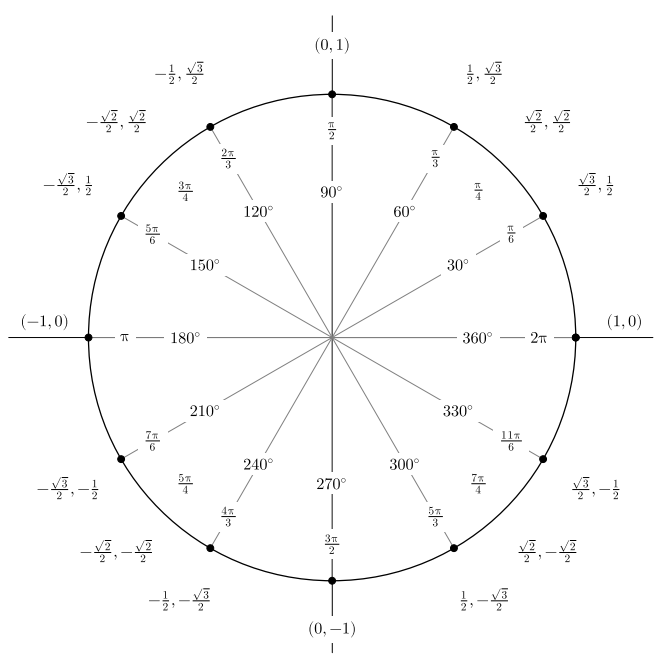
\includegraphics[width=\linewidth]{unit_cirlce.png}
% \end{center}
\begin{defbox}
    {Zeta-Funktion}
    $f(x)=\sum_{n=1}^\infty \dfrac{1}{n^s}$ divergiert für $s\le 1$ und konvergiert für $s>1$
\end{defbox}
\begin{tipbox}
{Arctan Werte}
\begin{center} 
 \begin{tabular}{c|cccc}
  deg & 0° & 30° & 45° & 60°\\
  \midrule
  x & 0 & $\frac{1}{3}\sqrt{3}$ & $1$ & $\sqrt{3}$ \\
  arctan(x) & 0 & $\frac{\pi}{6}$ & $\frac{\pi}{4}$ & $\frac{\pi}{3}$ \\
  
 \end{tabular}
\end{center}
\end{tipbox}
\begin{tbox}
    {$\log$ Rechenregeln}
    $\log_a (u\cdot v)=\log_a(u)+\log_a(v)$\\
    $\log_a(\frac{u}{v})=\log_a(u)-\log_b(v)$
\end{tbox}
\begin{tbox}
    {Umkehrfunktion Hilfe}
    $f(f^{-1}(x))=x$\\
    $(f^{-1})'(x)=\dfrac{1}{f'(f^{-1}(x))}$
\end{tbox}
\section{Tabellen}
\subsection{Grenzwerte}
\begin{center}
  \begin{tabularx}{\linewidth}{XX}
    \toprule
    $\limxi \frac{1}{x} = 0$ & $\limxi 1 + \frac{1}{x} = 1$ \\
    $\limxi e^x = \infty$ & $\limxn e^x = 0$ \\
    $\limxi e^{-x} = 0$ & $\limxn e^{-x} = \infty$ \\
    $\limxi \frac{e^x}{x^m} = \infty$ & $\limxn xe^x = 0$ \\
    $\limxi \ln(x) = \infty$ & $\limxo \ln(x) = -\infty$ \\
    $\limxi (1+x)^{\frac{1}{x}} = 1$ & $\limxo (1+x)^{\frac{1}{x}} = e$ \\
    $\limxi (1+\frac{1}{x})^b = 1$ & $\limxi n^{\frac{1}{n}} = 1$ \\
    $\lim_{x\to\pm\infty} (1 + \frac{1}{x})^x = e$ & $\limxi (1-\frac{1}{x})^x = \frac{1}{e}$ \\
    $\lim_{x\to\pm\infty} (1 + \frac{k}{x})^{mx} = e^{km}$ & $\limxi (\frac{x}{x+k})^x = e^{-k}$ \\
    $\limxo \frac{a^x -1}{x} = \ln(a), \newline \forall a > 0$ &
    $\limxi x^a q^x = 0, \newline \forall 0 \le q < 1$ \\
  \end{tabularx}
  \begin{tabularx}{\linewidth}{XX}
    $\limxo \frac{\sin x}{x} = 1$ & $\limxo \frac{\sin kx}{x} = k$\\
    $\limxo \frac{1}{\cos x} = 1$ & $\limxo \frac{\cos x -1}{x} = 0$ \\
    $\limxo \frac{\log 1 - x}{x} = -1$ & $\limxo x \log x = 0$\\
    $\limxo \frac{1 - \cos x}{x^2} = \frac{1}{2}$ & $\limxo \frac{e^x-1}{x} = 1$ \\
    $\limxo \frac{x}{\arctan x} = 1$ & $\limxi \arctan x = \frac{\pi}{2}$ \\
    $\limxo \frac{e^{ax}-1}{x} = a$ & $\limxo \frac{\ln(x+1)}{x} = 1$ \\
    $\lim_{x\to 1} \frac{\ln(x)}{x-1} = 1$ & $\limxi \frac{\log(x)}{x^a} = 0$ \\
    $\limxi \sqrt[x]{x} = 1$ & $\limxi \frac{2x}{2^x} = 0$ \\
    \bottomrule
  \end{tabularx}
\end{center}
\subsection{Ableitungen}
\begin{center}
  % the c>{\centering\arraybackslash}X is a workaround to have a column fill up all space and still be centered
  \begin{tabularx}{\linewidth}{c>{\centering\arraybackslash}Xc}
  \toprule
  $\mathbf{F(x)}$ & $\mathbf{f(x)}$ & $\mathbf{f'(x)}$ \\
  \midrule
  $\frac{x^{-a+1}}{-a+1}$ & $\frac{1}{x^a}$ & $\frac{a}{x^{a+1}}$ \\
  $\frac{x^{a+1}}{a+1}$ & $x^a \ (a \ne -1)$ & $a \cdot x^{a-1}$ \\
  $\frac{1}{k \ln(a)}a^{kx}$ & $a^{kx}$ & $ka^{kx} \ln(a)$ \\
  $\ln |x|$ & $\frac{1}{x}$ & $-\frac{1}{x^2}$ \\
  $\frac{2}{3}x^{3/2}$ & $\sqrt{x}$ & $\frac{1}{2\sqrt{x}}$\\
  $-\cos(x)$ & $\sin(x)$ & $\cos(x)$ \\
  $\sin(x)$ & $\cos(x)$ & $-\sin(x)$ \\
  $\frac{1}{2}(x-\frac{1}{2}\sin(2x))$ & $\sin^2(x)$ & $2 \sin(x)\cos(x)$ \\
  $\frac{1}{2}(x + \frac{1}{2}\sin(2x))$ & $\cos^2(x)$ & $-2\sin(x)\cos(x)$ \\
  \multirow{2}*{$-\ln|\cos(x)|$} & \multirow{2}*{$\tan(x)$} & $\frac{1}{\cos^2(x)}$  \\
  & & $1 + \tan^2(x)$ \\
  $\cosh(x)$ & $\sinh(x)$ & $\cosh(x)$ \\
  $\log(\cosh(x))$ & $\tanh(x)$ & $\frac{1}{\cosh^2(x)}$ \\
  $\ln | \sin(x)|$ & $\cot(x)$ & $-\frac{1}{\sin^2(x)}$ \\
  $\frac{1}{c} \cdot e^{cx}$ & $e^{cx}$ & $c \cdot e^{cx}$ \\
  $x(\ln |x| - 1)$ & $\ln |x|$ & $\frac{1}{x}$ \\
  $\frac{1}{2}(\ln(x))^2$ & $\frac{\ln(x)}{x}$ & $\frac{1 - \ln(x)}{x^2}$ \\
  $\frac{x}{\ln(a)} (\ln|x| -1)$ & $\log_a |x|$ & $\frac{1}{\ln(a)x}$ \\
  $ln(|\frac 1 x -1|)$ & $\frac 1 {x^2-x}$& $-\frac{2x-1}{(x^2-x)^2}$ \\
  \bottomrule
  \end{tabularx}
\end{center}
\subsection{Weitere Ableitungen}
\begin{center}
  \begin{tabularx}{\linewidth}{>{\centering\arraybackslash}X>{\centering\arraybackslash}X}
  \toprule
  $\mathbf{F(x)}$ & $\mathbf{f(x)}$ \\
  \midrule
  $\arcsin(x)$ & $\frac{1}{\sqrt{1 - x^2}}$ \\
  $\arccos(x)$ & $\frac{-1}{\sqrt{1 - x^2}}$ \\
  $\arctan(x)$ & $\frac{1}{1 + x^2}$ \\ 
  $x^x \ (x > 0)$ & $x^x \cdot (1 + \ln x)$ \\
  \bottomrule
  \end{tabularx}
\end{center}
\subsection{Integrale}
\begin{center}
 \begin{tabularx}{\linewidth}{>{\centering\arraybackslash}X>{\centering\arraybackslash}X}
  \toprule
  $\mathbf{f(x)}$ & $\mathbf{F(x)}$ \\
  \midrule
  $\int f'(x) f(x) \dx$ & $\frac{1}{2}(f(x))^2$ \\
  $\int \frac{f'(x)}{f(x)} \dx$ & $\ln|f(x)|$ \\
  $\int_{-\infty}^\infty e^{-x^2} \dx$ & $\sqrt{\pi}$ \\
  $\int (ax+b)^n \dx$ & $\frac{1}{a(n+1)}(ax+b)^{n+1}$ \\
  $\int x(ax+b)^n \dx$ & $\frac{(ax+b)^{n+2}}{(n+2)a^2} - \frac{b(ax+b)^{n+1}}{(n+1)a^2}$ \\
  $\int (ax^p+b)^n x^{p-1} \dx$ & $\frac{(ax^p+b)^{n+1}}{ap(n+1)}$ \\
  $\int (ax^p + b)^{-1} x^{p-1} \dx$ & $\frac{1}{ap} \ln |ax^p + b|$ \\
  $\int \frac{ax+b}{cx+d} \dx$ & $\frac{ax}{c} - \frac{ad-bc}{c^2} \ln |cx +d|$ \\
  $\int \frac{1}{x^2+a^2} \dx$ & $\frac{1}{a} \arctan \frac{x}{a}$ \\
  $\int \frac{1}{x^2 - a^2} \dx$ & $\frac{1}{2a} \ln\left| \frac{x-a}{x+a} \right|$ \\
  $\int \sqrt{a^2+x^2} \dx $ & $\frac{x}{2}f(x) + \frac{a^2}{2}\ln(x+f(x))$ \\
  \bottomrule
 \end{tabularx}
\end{center}
\section{Quellen}
Das Layout, der Einheitskreis und die Tabellen wurden von dem Cheatsheet von Julian Steinmann (https://github.com/XYQuadrat/eth-cheatsheets/blob/main/analysis1/analysis1.tex) übernommen. Die Sätze, Bemerkungen und Definition stammen zum Grossteil aus eigenen Notizen von der Vorlesung und wurden mit Hilfe des Skripts ergänzt.
\end{document}
